% Graphic for TeX using PGF
% Title: /home/lihram/git/github.com/lihram/p8-matrix-p2p/report/graphics/client-server.dia
% Creator: Dia v0.97.3
% CreationDate: Tue Mar 31 12:48:39 2020
% For: lihram
% \usepackage{tikz}
% The following commands are not supported in PSTricks at present
% We define them conditionally, so when they are implemented,
% this pgf file will use them.
\ifx\du\undefined
  \newlength{\du}
\fi
\setlength{\du}{15\unitlength}
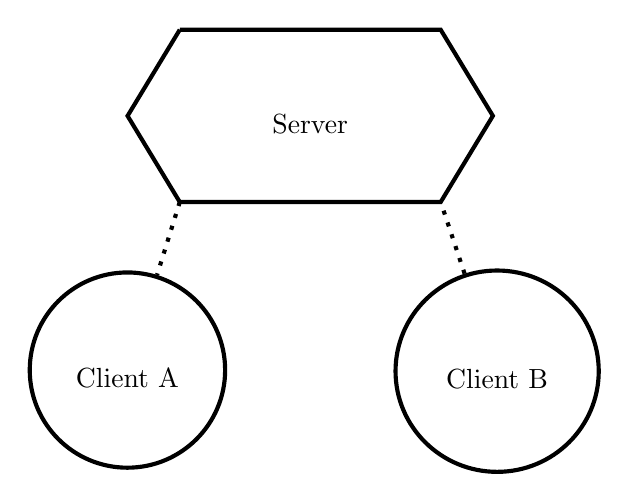
\begin{tikzpicture}
\pgftransformxscale{1.000000}
\pgftransformyscale{-1.000000}
\definecolor{dialinecolor}{rgb}{0.000000, 0.000000, 0.000000}
\pgfsetstrokecolor{dialinecolor}
\definecolor{dialinecolor}{rgb}{1.000000, 1.000000, 1.000000}
\pgfsetfillcolor{dialinecolor}
\pgfsetlinewidth{0.100000\du}
\pgfsetdash{}{0pt}
\pgfsetdash{}{0pt}
\pgfsetbuttcap
\pgfsetmiterjoin
\pgfsetlinewidth{0.100000\du}
\pgfsetbuttcap
\pgfsetmiterjoin
\pgfsetdash{}{0pt}
\definecolor{dialinecolor}{rgb}{1.000000, 1.000000, 1.000000}
\pgfsetfillcolor{dialinecolor}
\pgfpathmoveto{\pgfpoint{4.257143\du}{0.800000\du}}
\pgfpathlineto{\pgfpoint{10.542857\du}{0.800000\du}}
\pgfpathlineto{\pgfpoint{11.800000\du}{2.875000\du}}
\pgfpathlineto{\pgfpoint{10.542857\du}{4.950000\du}}
\pgfpathlineto{\pgfpoint{4.257143\du}{4.950000\du}}
\pgfpathlineto{\pgfpoint{3.000000\du}{2.875000\du}}
\pgfpathlineto{\pgfpoint{4.257143\du}{0.800000\du}}
\pgfusepath{fill}
\definecolor{dialinecolor}{rgb}{0.000000, 0.000000, 0.000000}
\pgfsetstrokecolor{dialinecolor}
\pgfpathmoveto{\pgfpoint{4.257143\du}{0.800000\du}}
\pgfpathlineto{\pgfpoint{10.542857\du}{0.800000\du}}
\pgfpathlineto{\pgfpoint{11.800000\du}{2.875000\du}}
\pgfpathlineto{\pgfpoint{10.542857\du}{4.950000\du}}
\pgfpathlineto{\pgfpoint{4.257143\du}{4.950000\du}}
\pgfpathlineto{\pgfpoint{3.000000\du}{2.875000\du}}
\pgfpathlineto{\pgfpoint{4.257143\du}{0.800000\du}}
\pgfusepath{stroke}
% setfont left to latex
\definecolor{dialinecolor}{rgb}{0.000000, 0.000000, 0.000000}
\pgfsetstrokecolor{dialinecolor}
\node at (7.400000\du,3.069043\du){Server};
\definecolor{dialinecolor}{rgb}{1.000000, 1.000000, 1.000000}
\pgfsetfillcolor{dialinecolor}
\pgfpathellipse{\pgfpoint{2.996636\du}{8.998318\du}}{\pgfpoint{2.353364\du}{0\du}}{\pgfpoint{0\du}{2.351682\du}}
\pgfusepath{fill}
\pgfsetlinewidth{0.100000\du}
\pgfsetdash{}{0pt}
\pgfsetdash{}{0pt}
\pgfsetmiterjoin
\definecolor{dialinecolor}{rgb}{0.000000, 0.000000, 0.000000}
\pgfsetstrokecolor{dialinecolor}
\pgfpathellipse{\pgfpoint{2.996636\du}{8.998318\du}}{\pgfpoint{2.353364\du}{0\du}}{\pgfpoint{0\du}{2.351682\du}}
\pgfusepath{stroke}
% setfont left to latex
\definecolor{dialinecolor}{rgb}{0.000000, 0.000000, 0.000000}
\pgfsetstrokecolor{dialinecolor}
\node at (2.996636\du,9.192371\du){Client A};
\definecolor{dialinecolor}{rgb}{1.000000, 1.000000, 1.000000}
\pgfsetfillcolor{dialinecolor}
\pgfpathellipse{\pgfpoint{11.902500\du}{9.025000\du}}{\pgfpoint{2.447500\du}{0\du}}{\pgfpoint{0\du}{2.425000\du}}
\pgfusepath{fill}
\pgfsetlinewidth{0.100000\du}
\pgfsetdash{}{0pt}
\pgfsetdash{}{0pt}
\pgfsetmiterjoin
\definecolor{dialinecolor}{rgb}{0.000000, 0.000000, 0.000000}
\pgfsetstrokecolor{dialinecolor}
\pgfpathellipse{\pgfpoint{11.902500\du}{9.025000\du}}{\pgfpoint{2.447500\du}{0\du}}{\pgfpoint{0\du}{2.425000\du}}
\pgfusepath{stroke}
% setfont left to latex
\definecolor{dialinecolor}{rgb}{0.000000, 0.000000, 0.000000}
\pgfsetstrokecolor{dialinecolor}
\node at (11.902500\du,9.219053\du){Client B};
\pgfsetlinewidth{0.100000\du}
\pgfsetdash{{\pgflinewidth}{0.200000\du}}{0cm}
\pgfsetdash{{\pgflinewidth}{0.200000\du}}{0cm}
\pgfsetbuttcap
{
\definecolor{dialinecolor}{rgb}{0.000000, 0.000000, 0.000000}
\pgfsetfillcolor{dialinecolor}
% was here!!!
\definecolor{dialinecolor}{rgb}{0.000000, 0.000000, 0.000000}
\pgfsetstrokecolor{dialinecolor}
\draw (11.118780\du,6.676105\du)--(10.542857\du,4.950000\du);
}
\pgfsetlinewidth{0.100000\du}
\pgfsetdash{{\pgflinewidth}{0.200000\du}}{0cm}
\pgfsetdash{{\pgflinewidth}{0.200000\du}}{0cm}
\pgfsetbuttcap
{
\definecolor{dialinecolor}{rgb}{0.000000, 0.000000, 0.000000}
\pgfsetfillcolor{dialinecolor}
% was here!!!
\definecolor{dialinecolor}{rgb}{0.000000, 0.000000, 0.000000}
\pgfsetstrokecolor{dialinecolor}
\draw (4.257143\du,4.950000\du)--(3.710749\du,6.704831\du);
}
\end{tikzpicture}
